\documentclass[12pt,spanish]{article}
\usepackage[spanish]{babel}
\usepackage{graphicx}
\usepackage{multirow}
\usepackage[hidelinks]{hyperref}
\usepackage{caption}
\usepackage{multirow}
\usepackage{multicol}
\usepackage[outputdir=build]{minted}
\usepackage{float}
\usepackage{array}
\graphicspath{ {../img/} {../../LaTeX/img/} {/home/csp98/latex/img/}}
\selectlanguage{spanish}
\usepackage[utf8]{inputenc}
\usepackage{graphicx}
\usepackage[a4paper,left=3cm,right=2cm,top=2.5cm,bottom=2.5cm]{geometry}
\newtheorem{ppio}{Principio }
\makeindex

\begin{document}
\begin{titlepage}

\newlength{\centeroffset}
\setlength{\centeroffset}{-0.5\oddsidemargin}
\addtolength{\centeroffset}{0.5\evensidemargin}
\thispagestyle{empty}

\noindent\hspace*{\centeroffset}
\begin{minipage}{\textwidth}

\centering
\includegraphics[width=0.9\textwidth]{logo_ugr.jpg}\\[1.4cm]

\textsc{ \Large Algorítmica\\[0.2cm]}
\textsc{GRADO EN INGENIERÍA INFORMÁTICA}\\[1cm]

{\Huge\bfseries Ejercicio de clase\\}
\noindent\rule[-1ex]{\textwidth}{3pt}\\[3.5ex]
{\large\bfseries Divide y Vencerás}
\end{minipage}

\vspace{1.5cm}
\noindent\hspace*{\centeroffset}
\begin{minipage}{\textwidth}
\centering

\textbf{Autores}\\ {Carlos Sánchez Páez}\\[2.5ex]
\includegraphics[width=0.3\textwidth]{etsiit_logo.png}\\[0.1cm]
\vspace{1.5cm}
\includegraphics[width=0.5\textwidth]{decsai.jpg}\\[0.1cm]
\vspace{1cm}
\textsc{Escuela Técnica Superior de Ingenierías Informática y de Telecomunicación}\\
\vspace{1cm}
\textsc{Curso 2017-2018}
\end{minipage}
\end{titlepage}
\tableofcontents
\thispagestyle{empty}
\listoftables
\newpage
\setcounter{page}{1}

\section{Enunciado}
\large{Implementar un algoritmo sencillo para calcular el valor máximo de un vector y otro basado en divide y vencerás. Realizar un estudio empírico e híbrido de su eficiencia.}

\section{Resolución}

\subsection{Algoritmo desarrollado}
Para resolver el ejercicio he implementado el siguiente programa:
\begin{minted}[linenos]{c++}
#include <iostream>
#include <stdlib.h>  
#include <time.h>      
#include <climits>

using namespace std;

int hallarMaximo(const int *v, const int inicio, const int fin) {
	int max = v[inicio];
	for (int i = inicio + 1; i < fin; i++)
		if (v[i] > max)
			max = v[i];
	return max;
}

int hallarMaximoDyV(const int *v,const int i,const int j){
	if(i==j){
		return v[i];
	}
	else{
		int mitad=(i+j)/2;
		int max_izquierda=hallarMaximoDyV(v,i,mitad);
		int max_derecha=hallarMaximoDyV(v,mitad+1,j);
		if(max_izquierda>max_derecha)
			return max_izquierda;
		else
			return max_derecha;
	}
}

int main(int argc, char **argv) {
	if (argc != 2) {
		cerr << "Falta el tamaño del vector.";
		exit(-1);
	}

	int tam = atoi(argv[1]);
	int *v = new int[tam];
	int max;
	clock_t tantes;   
	clock_t tdespues; 

	//Inicializar vector con valores aleatorios
	srand (time(NULL));

	for (int i = 0; i < tam; i++)
		v[i] = rand() ;

	//Algoritmo sencillo
	
	cout<<"\t\tTamaño "<<tam<<endl;
	tantes = clock();
	max = hallarMaximo(v, 0, tam);
	tdespues = clock();
	cout << "Algoritmo sencillo:\tMáximo: " << max 
	<< "\tTiempo: " << ((double)(tdespues - tantes))
	 / CLOCKS_PER_SEC << endl;
	 
	//Algoritmo DyV

	tantes = clock();
	max = hallarMaximoDyV(v, 0,tam);
	tdespues = clock();
	cout << "Algoritmo DyV:\tMáximo:" << max 
	<< "\tTiempo: " << ((double)(tdespues - tantes)) 
	  / CLOCKS_PER_SEC << endl;
}
\end{minted}
\newpage
\subsection{Método básico}

El método básico sigue el siguiente algoritmo:
\begin{enumerate}
\item Asigno el máximo al primer elemento del vector
\item Itero desde $v[1]$ hasta $v[tam]$
	\begin{itemize}
		\item Si encuentro un elemento mayor que el máximo almacenado, lo 			sustituyo.
	\end{itemize}
	\item Devuelvo el máximo.
\end{enumerate}
\begin{minted}[linenos]{c++}
int hallarMaximo(const int *v, const int inicio, const int fin) {
	int max = v[inicio];
	for (int i = inicio + 1; i < fin; i++)
		if (v[i] > max)
			max = v[i];
	return max;
}
	...
	max = hallarMaximo(v, 0, tam);
\end{minted}

Como vemos, su eficiencia \emph{teórica} es $O(n)$.

\subsection{Método Divide y Vencerás}

En el método Divide y Vencerás hacemos lo siguiente:
\begin{enumerate}
\item Caso base: i=j. Devolvemos $v[i]=v[j]$
\item Lanzamos el algoritmo dos veces, desde $i$ a la mitad y desde la mitad al final.
\item Devolvemos el máximo de entre las dos ejecuciones anteriores.
\end{enumerate}

\begin{minted}[linenos]{c++}
int hallarMaximoDyV(const int *v,const int i,const int j){
	if(i==j){
		return v[i];
	}
	else{
		int mitad=(i+j)/2;
		int max_izquierda=hallarMaximoDyV(v,i,mitad);
		int max_derecha=hallarMaximoDyV(v,mitad+1,j);
		if(max_izquierda>max_derecha)
			return max_izquierda;
		else
			return max_derecha;
	}
}
	...
	max = hallarMaximoDyV(v, 0,tam);
\end{minted}
Como vemos, su eficiencia es $O(\frac{n}{2})=O(n)$
\subsection{Estudio de eficiencia}

\subsubsection{Eficiencia empírica}

Para realizar un estudio de la eficiencia empírica, ejecutaremos el programa 25 veces con tamaños ascendentes mediante un script:

\begin{minted}[linenos]{bash}

#!/bin/bash                                                                     
if [ $# -eq 3 ]
then
i="0"
tam=$2
#Primer argumento: programa a ejecutar                                          
#Segundo argumento: tamaño inicial                                              
#Tercer argumento : incremento                                                  
while [ $i -lt 25 ]
do
        ./$1 $tam >> ./$1.dat
        i=$[$i+1]
        tam=$[$tam+$3]
done
else
echo "Error de argumentos"
fi

\end{minted}
%$

\begin{table}[H]
\centering
\begin{tabular}{|c|c|c|}
\hline
\textbf{Tamaño inicial} & \textbf{Tamaño final} & \textbf{Incremento} \\
\hline
100.000.000 & 340.000.000 &10.000.000 \\
\hline
\end{tabular}
\caption{Parámetros de ejecución}
\end{table}

Los tiempos obtenidos son los siguientes:

\begin{table}[H]
\centering
\begin{tabular}{|c|c|c|}
\hline
\textbf{Tamaño del vector} &\textbf{Algoritmo sencillo} & \textbf{Algoritmo DyV}\\
\hline
1.000.000 & 0.002843 & 0.01785 \\
\hline
1.100.000 & 0.003078 & 0.019833 \\
\hline
1.200.000 & 0.003348 & 0.021738 \\
\hline
1.300.000 & 0.003672 & 0.023498 \\
\hline
1.400.000 & 0.00399 & 0.025195 \\
\hline
1.500.000 & 0.004231 & 0.026859 \\
\hline
1.600.000 & 0.004494 & 0.02824 \\
\hline
1.700.000 & 0.004768 & 0.030195 \\
\hline
1.800.000 & 0.005065 & 0.031905 \\
\hline
1.900.000 & 0.005365 & 0.03421 \\
\hline
2.000.000 & 0.005717 & 0.035741 \\
\hline
2.100.000 & 0.005959 & 0.036774 \\
\hline
2.200.000 & 0.006238 & 0.039702 \\
\hline
2.300.000 & 0.00655 & 0.041812 \\
\hline
2.400.000 & 0.006852 & 0.043164 \\
\hline
2.500.000 & 0.007097 & 0.04456 \\
\hline
2.600.000 & 0.007376 & 0.047041 \\
\hline
2.700.000 & 0.007694 & 0.048758 \\
\hline
2.800.000 & 0.007935 & 0.050333 \\
\hline
2.900.000 & 0.00823 & 0.051901 \\
\hline
3.000.000 & 0.008527 & 0.053997 \\
\hline
3.100.000 & 0.008772 & 0.055266 \\
\hline
3.200.000 & 0.009132 & 0.056647 \\
\hline
3.300.000 & 0.009391 & 0.05865 \\
\hline
3.400.000 & 0.009629 & 0.060409 \\
\hline
\end{tabular}
\caption{Tiempos de ejecución (s)}
\end{table}

\begin{figure}[H]
\centering
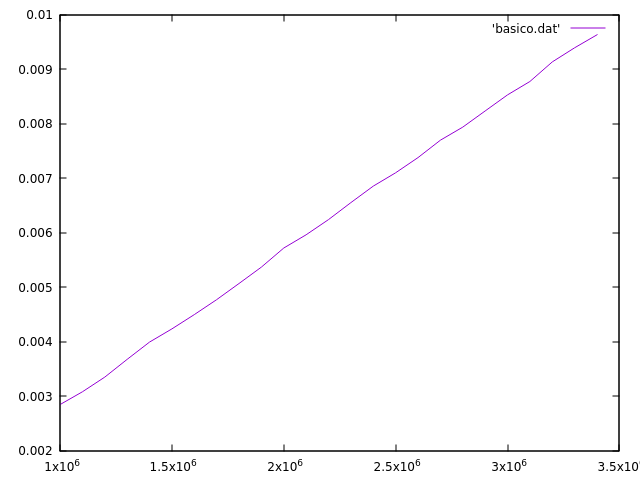
\includegraphics[scale=0.85]{empirica_basico.png}
\caption{Eficiencia empírica. Algoritmo básico}
\end{figure}

\begin{figure}[H]
\centering
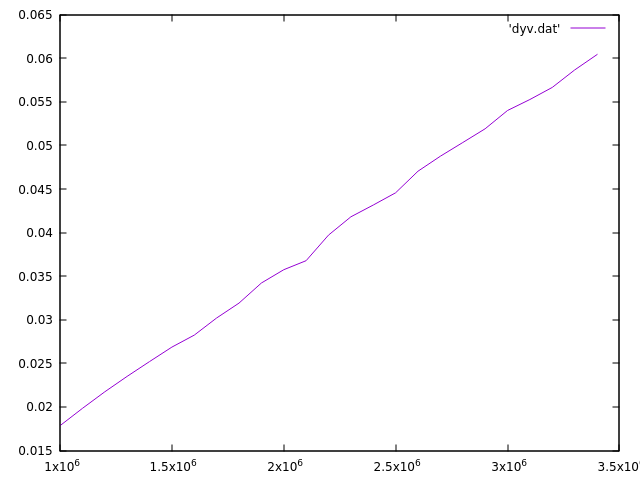
\includegraphics[scale=0.85]{empirica_dyv.png}
\caption{Eficiencia empírica. Algoritmo Divide y Vencerás}
\end{figure}

\subsubsection{Eficiencia híbrida}
Para esta sección, haremos una regresión mediante \emph{gnuplot} de los datos empíricos obtenidos a la función $f(x)=a \cdot x$ para hallar la constante oculta.

\begin{table}[H]
\centering
\begin{tabular}{|c|c|c|}
\hline
\textbf{Algoritmo} & \textbf{Valor de la constante oculta} & \textbf{Porcentaje de error} \\
\hline
Básico & 2.83765e-09 & 0.09622\% \\
\hline
Divide y Vencerás & 1.78876e-08 & 0.1751\%\\
\hline
\end{tabular}
\caption{Bondad del ajuste}
\end{table}

\begin{figure}[H]
\centering
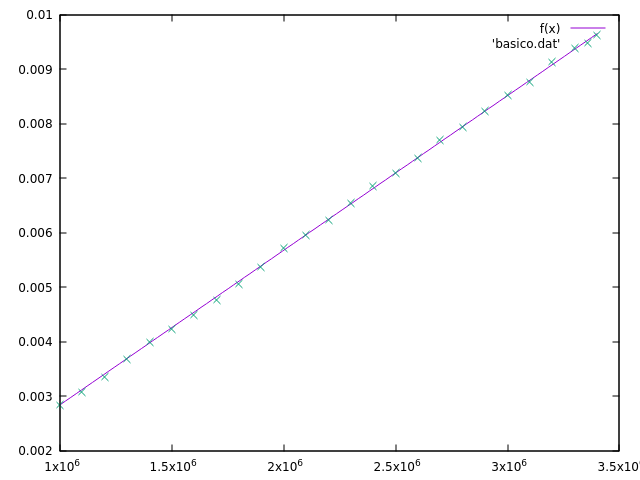
\includegraphics[scale=0.85]{hibrida_basico.png}
\caption{Eficiencia híbrida. Algoritmo básico}
\end{figure}

\begin{figure}[H]
\centering
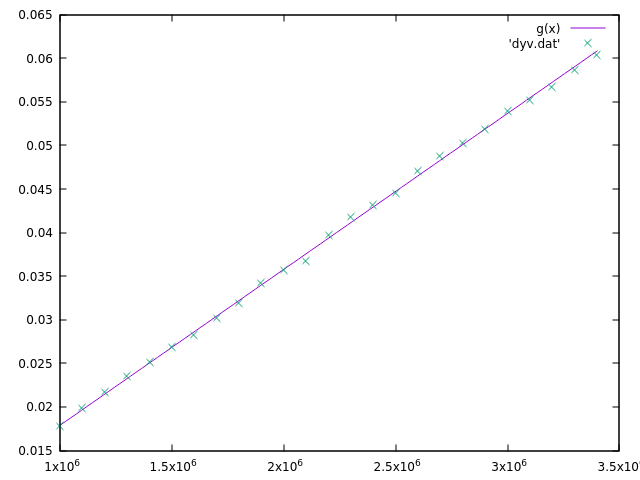
\includegraphics[scale=0.85]{hibrida_dyv.png}
\caption{Eficiencia híbrida. Algoritmo Divide y Vencerás}
\end{figure}

\subsection{Conclusiones}
Como podemos ver, gracias al método \emph{Divide y Vencerás} conseguimos rebajar la constante oculta del algoritmo inmediato. Sin embargo, sigue siendo mejor utilizar el algoritmo básico debido a los costes de la recursión que requiere Divide y Vencerás.
\end{document}
